The previous chapter has presented the four policy making theories that are considered. It also reflected on the different concepts presented in the theories and how, when possible, these concepts could be used together. This chapter builds on that reflection and presents the different concepts that will be used for this thesis. Most of the concepts are taken directly from one of the four theories and made compatible for all theories. For the concepts that have been specifically mentioned during the validation interview, there will be a mention of the feedback that was obtained from the researchers contacted.

The order in which the concepts are ordered is chosen such that the wider concepts are mentioned first. \autoref{sec:policyProcess} presents the policy process that is used within this model. It is followed by the selection of the actors in \autoref{sec:actors} and a mention on the concept of political affiliation in \autoref{sec:affiliation} and the policy network in \autoref{sec:policyNetwork}. The description of the actor's beliefs system is then done in \autoref{sec:beliefTree} followed by an explanation of the policy instruments in \autoref{sec:policyInstruments} as approached within this thesis. Then the concepts that are related specifically to one policy making theory at a time are mentioned in \autoref{sec:PMTConcepts}. These concepts related to the three streams theory, the advocacy coalition framework, the feedback theory and the diffusion theory.

% Steps for each of these parts:
% 1. Mention the history of the concepts (from the literature)
% 2. Explain the approach chosen within the context of this thesis

%
%\section{The System and Super-System}
%\label{sec:systemSuperssystem}


%
\section{The Policy Process}
\label{sec:policyProcess}

The first and most important concept to consider is the policy process. The process used usually follows the policy cycle. The steps are then given as being: the agenda setting process, the formulation of the policy, the implementation of the policy and the review of the policy \cite{lester2000public, stewart2007public, palumbo1987symposium, hogwood1984policy, hill2016public}. As mentioned before, the three streams theory goes further by proposing a three step process with the agenda setting, the decision making process and the implementation. The approach used here is a mix of these approaches. The policy emergence model that is to be built for this thesis can be considered to span the agenda setting and the decision making or policy formulation steps. The rest of the process is considered to be part of the technical model. It contains the implementation of the policy and the review of the policy. The technical model is not within the scope of this thesis. It is a model that is case study specific and that describes how the world run. It could for example be a public transportation model of a specific city.

This approach is further enhanced to consider the possibility of several levels of aggregation within the case study considered. The policy cycle used to model the policy emergence is therefore approached as a modular process. This approach is outlined in \autoref{fig:Conceptualisation_V3-01}. For all variation of this approach, it is always split into two main parts: the technical model and the policy emergence model. The technical model is the part which define the current states of the world to the policy emergence model. The policy emergence model uses these states to produce, through a decision making process, a certain policy instrument. This policy instrument is chosen by the actors present in the model. In a 2-step model, the policy emergence model is only one step long. The actors just decide on a policy instrument that will need to be implemented in the technical model to solve the perceived problems. If the actors agree on an instrument, that instrument is implemented in the technical model. If not, the technical model runs without a new instrument in the next cycle.

\begin{figure}
\centering
\includegraphics[scale=0.33, angle = 0]{figures/Conceptualisation_V3-01}
\caption{Policy process cycle as presented in the conceptualisation for a 2, 3 and 4-step cycle. In grey are the processes performed by the technical model, in green are the processes performed by the policy emergence model. }
\label{fig:Conceptualisation_V3-01}
\end{figure}

 
Using this approach, it is also possible for the modeller to add steps to the policy emergence model if needed. A 3-step model can therefore be considered. In the first step of the policy emergence level, the actors first decide on what will be on the agenda. Once they have chosen the agenda, the actors choose an instrument that relates to what is on the agenda in the second step. This step happens at a lower level of aggregation. This allows more depth to the emergence process. This 3-step model is the one considered within the three streams theory \citep{zahariadis2014ambiguity}. This can be furthered by adding another step to obtain a 4-step model. In this case, in the first step of the technical model, the actors have to specify a first agenda. Having this first agenda, they can limit their number of issues considered for the next phase to the issues related to their obtained first agenda. A second agenda is then formulated based on the issues they can consider. In the third and last step, they choose an instrument based on the second agenda constructed. This approach can be extended to $n$ amount of steps but it only increases the number of levels considered and hence the complexity of the model.
 
For the remainder of this report, the 3-step model is considered. The first step of the policy emergence model is called the agenda setting process while the second step is called the policy formulation process. The third step is the technical model. From now on, all models will assume this 3-step model except if otherwise stated. With this 3-step model, it is assumed that the models constructed are already at the subsystem level according to the ACF definition \citep{jenkins2014advocacy, mccool1998subsystem}. This has for consequences that all actors that are included within the model have an interest in the issues being addressed. In turn, this leads to the fact that every actors can be part of a group throughout the model when the three streams theory or the ACF are being used.

%
\section{The Actors}
\label{sec:actors}

The number of actor types considered within this model is limited to five. They are divided into two main categories. First, the passive actor category is composed of the electorate. Passive actors cannot actively perform actions on other actors. The second category is composed of the active actors. These are the policy makers, the policy entrepreneurs, the external parties and the policy brokers. These active actors can perform actions on other actors. Only one type of actor, the external parties, is an ambiguous actor as it performs active actions but is also forced with passive actions. This is detailed later on.

%-
\subsection{The electorates}

The electorate actor represents the voting general public. The electorate is implemented as several actors for which, each actor corresponds to one sector of the electorate. In turn, one sector of the electorate corresponds to one political affiliation. The aim is to represent the overall political balance that is present in the case being studied. The important feature of the electorate is its representation. This parameter is an indication of the amount of potential voters in percentage that is represented by this electorate actor. This can vary over time and will have an impact on the rest of the model as is explained later on.

%-
\subsection{The policy makers}

The first type of active actor considered, and the most important one, is the policy maker. The policy makers are required for the policy emergence process. They are the only actors that have decision making power \citep{zahariadis2014ambiguity}. They are therefore the ones that can select the agenda or the instrument that can be implemented in the world. They can also be influenced by other actors present in the model. The policy makers are provided with resources every for every time period. These resources represent their political but also financial resources. They can be associated with the concepts of energy and money within the three streams theory \citep{zahariadis2014ambiguity}. The resources given to the policy makers are used to perform actions on other actors.

Each policy maker is also associated with a political affiliation. Depending on the representation of the associated electorate for the policy maker's affiliation, the amount of resources that will be assigned will vary. A policy maker associated to an electorate with a high representation will be provied with more resources than one with a low representation. This helps represent the power provided by the voters to the policy makers. Elections that lead to a change in electorate representation will also lead to a change in the amount of resources assigned to each policy makers and therefore their abilities to perform actions.

%-
\subsection{The policy entrepreneurs}

The second type of active actor considered is the policy entrepreneur. The policy entrepreneurs are actors that are present within the system to further certain interests. They are present in both the three streams theory and the advocacy coalition framework \citep{zahariadis2014ambiguity, jenkins2014advocacy}. Policy entrepreneurs represent lobbyists, non-governmental organisations but also governmental bodies. Similarly to the policy makers, policy entrepreneurs all have a certain political affiliation. Furthermore, they have a certain amount of resources that they can use to perform actions.

A current assumption on the distribution of the policy entrepeneur resources is that they are related to affiliation like for the policy makers. This means that entrepreneurs linked by affiliation to a large electorate representation will have more resources for each time period. This assumption is not always perfect. In some instances, it will be important to assign resources independently from the affiliation. In some very specific cases, the amount of resources should be inversely proportionate to the affiliation. This is the case for the National Rifle Association for example which sees its donations drop when a Republican president enters the White House. How the resources are assigned for these entrepreneurs is linked to the case study considered.

%-
\subsection{The external parties}

The third type of active actor considered is the external party. The external parties are actors that help bridge the gap between the real world and the actors in the policy network. The external parties represent actors such as the media, but also research institute or academic institutions  \citep{birkland2004world, van2000new, mccombs1972agenda, cook1983media, kosicki1993problems, van1993domestic}. These are the only actors that have access to the true states of the world independently from any political influence. They are the actors that inform other actors about the states of the world. The external parties are however not perfect. All external parties are not interested in all issues within the model, they have selective interests. This can have an impact on the information they relay to the other actors in the model. To quantify this impact, the external parties also have affiliations.

The external parties can also perform more active actions and infuence the other actors in the same way as policy entrepreneurs do. They therefore provided with resources which are, once again, assigned depending on affiliation. The same assumption as the one made for the policy entrepreneurs on the amount of resources assigned is made. It could again be argued that resources should be assigned inversely to the affiliation representation. An clear and current example that can be taken to illustrate this point is the current boom in media revenue for media opposing the current US president. This is not done here and can be the topic of subsequent research.

For the policy makers and the external parties, it was briefly mentioned that both type of actors can perform actions on other actors in a similar way to the policy entrepreneur. The approach chosen here is to illustrate that all actors are, in essence, policy entrepreneurs attempting to further their own interest. The reason why the type of actors are differentiated is to make clear that policy makers have additional decision making actions compared to the entrepreneurs and external parties are actors that also have access to the true states of the world. The different actions available to the policy entrepreneurs and the other actors are detailed in the next chapter.

%-
\subsection{The policy brokers}

The final type of active actor considered is the policy broker. This is not a normal type of actor as any of the previously mentioned actor can become brokers. Policy brokers are a temporary status provided to the actors. This status extends the amount of actions that the actor can perform. The policy broker stems from the advocacy coalition framework \citep{ingold2011treating, ingold2011network, jenkins2014advocacy, henry2011belief}. The role of the policy broker is to connect actors that were not previously connected or that had a low awareness of each other. The aim of such actions is to enhance the policy learning present in the system. Policy brokers are selected amongst other actors based on their policy network connections and their resources. Two types of policy broker can be distinguished. The first type is a policy broker that will tend to connect actors in such a way that the policy broker's interest are also advanced. In that case the policy broker is playing an advocacy role \citep{bardach1998getting}. Neutral facilitator can also be considered in which case the policy broker will connect any actors together regardless of their interests.

In her validation feedback, Dr. Ingold mentioned that policy brokers tend to be policy makers. However, for flexibility, this conceptualisation allows any active actor to become a policy broker. Whether policy makers are more likely to become policy brokers will stem from the simulation and the tuning of the model. Finally, the use of policy brokers within the model is optional. Furthremore, although it is technically possible to use policy brokers all the time, it is advised to only use policy brokers with the advocacy coalition framework to better match the literature.

%
\section{The Affiliations}
\label{sec:affiliation}

As hinted at earlier on, each actor is associated to an affiliation. This affiliation represent the political beliefs which characterises a certain actor. The importance of affiliation arises when considering the inter-actions between the actors. Actors with similar affiliations are more likely to interact with each other while actors with differing affiliations are less likely to interact. This level of interaction is defined through an affiliation network. This network defines the reduction in interaction between the different affiliations. For example, affiliations distant from each other in ideology will have a very low coefficient to reduce the importance of their interactions.

%
\section{The Policy Network}
\label{sec:policyNetwork}

The policy network, shown in \autoref{fig:Conceptualisation_V3-03}, is the network that spans the entire model and which connects all active actors (the policy makers, the policy entrepreneurs and the external parties). This network is composed of undirected links representing the level of awareness that actors have of one another. The network affects the actions that the actors can perform and the impact of these actions. It can also be used to represent the lack of connection between different actors. In some cases, actors are not aware of other actors present in the network or simply do not have any connection to them.

The network links are not static over time. The level of awareness reduces as time passes by according to a certain awareness decay coefficient. This means that actors not engaging with each other will see their perceived awarness of each other diminish over time. This means that the each of the links require upkeep from the actors so that they remain in contact and aware of each other's presence in the network. This maintenance of the network is done through specific actions that the actors have at their disposition. This is detailed in the next chapter. Note that if actors interact with each other, the decay in awarness will be halted for a certain time period depending on the interaction.

The policy network also introduces the conflict level aspect between the different actors on specific issues \citep{jenkins2014advocacy}. The conflict level influences whether actors are likely to speak to each other. Three levels of conflict levels are identified for each issue between each actor: low, average and high. The conflict level is defined on a per issue basis for each link between two agents. It is calculated depending on the different in beliefs for each issue. For large difference in beliefs, the conflict level will be high while for low difference, the conflict level will be low. As stated in \cite{jenkins2014advocacy}, average conflict levels will lead to actors being more likely to interact with one another, high conflict level will lead to a small chance of two actors interacting with each other while a low conflict level will lead to an average probability of interaction.

\begin{figure}
\centering
\includegraphics[scale = 0.33, angle = 0]{figures/Conceptualisation_V3-03}
\caption{Illustration of the policy network using 3-step models.}
\label{fig:Conceptualisation_V3-03}
\end{figure}

%
\section{The Belief Tree}
\label{sec:beliefTree}

This belief tree is what constitutes the 'brain' of the different actors present in the model. It is an attribute that all actors have and which is used to define their beliefs on the different issues. This applies to the actors in the ACF but also in the other three theories. The belief tree structure is based on the three layered system that is used to describe the actor's belief in \cite{jenkins2014advocacy}. The number of layers is dependent on the number of levels that are considered by the modeller. In a 2-step model, the belief tree would only have two layers while in a 4-step model, it would require four. The reasoning behind this will become apparent throughout this section.

The representation of the tree that is used within this conceptualisation is shown in \autoref{fig:BeliefTreeConceptualisation-01}. The top layer represent the principle beliefs of the actor. These are beliefs that are meant to only change over long periods of time and are unlikely to be affected by day to day problems. The second layer represents the policy core beliefs of the actor which are easier to change over time. As defined in \cite{jenkins2014advocacy}, the policy core beliefs "are bound by scope and topic" to the system considered. Finally, the third and bottom layer of the belief tree represents the secondary beliefs of the actors. The secondary beliefs tend to be associated with detailed issues for which the actors are more likely to change their minds over short periods of time. Secondary beliefs are the lowest beliefs in the tree. They are the beliefs on which policy instrument will directly act when being impelemented. The same belief tree structure is used for all actors. The difference between the actors is the values associated to the different issues present in the tree.

To further this explanation, if the modeller were to choose a 4-step model, then three would be composed of four layers as mentioned earlier. The highest beliefs in the tree would remain principle beliefs. The second level could be called the policy core beliefs 1 and the third level policy core beliefs 2. The lowest level would remain filled with secondary beliefs, as by definition, these are the beliefs that are impacted directly by a policy instrument. The two policy core levels would be at a different level.

Depending on the level of aggregation chosen by the modeller for the system, the deep core beliefs as highlighted in the literature \cite{jenkins2014advocacy} could possible match with the principle beliefs. This shoud highlight the flexibility of the approach chosen but also the need for the modeller to choose the tree and its corresponding structure coherently with the system studied.
 
\begin{figure}
\centering
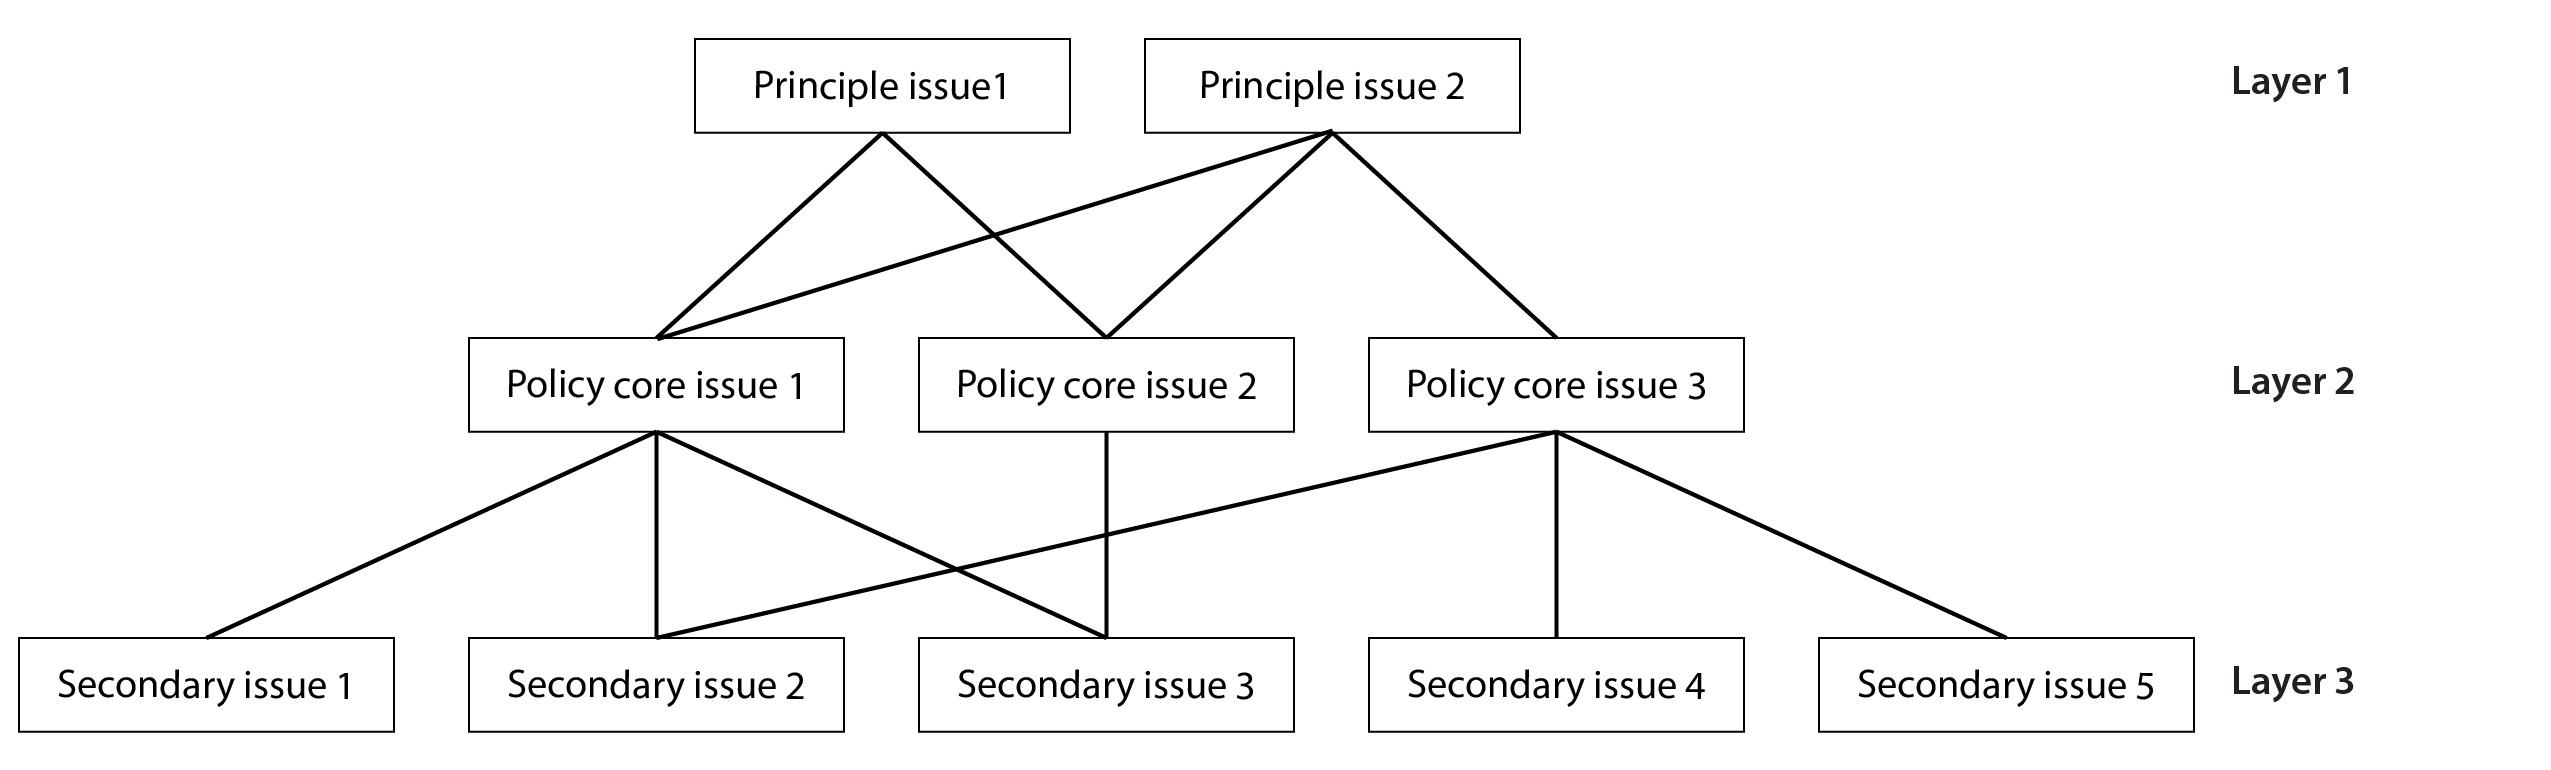
\includegraphics[scale = 0.33, angle = 0]{figures/BeliefTreeConceptualisation-01}
\caption{Conceptual representation of the belief system tree hierarchy. Note that not all possible causal relations are illustrated.}
\label{fig:BeliefTreeConceptualisation-01}
\end{figure}
 
Within the conceptualisation, these different belief layers are associated to specific parts of the model. The principle beliefs are associated to what is called principle issues. These are very high level issues that the actors must consider. They are for example, and this will depend on the model considered, the economy, security or the environment. The policy core beliefs are associated to policy core issues. These are intermediate descriptions of the system which outline large swath of the model but a level lower than wide ranging issues used for principle issues. Finally, the third layer is composed of the secondary issues. These are very low and detailed issue that can be considered to be the parts of the model. In the case of public transportation, this could be the use of a metro or the use of car infrastructure. Secondary issues are the ones on which policy instruments will act. It is therefore important that the secondary issues be modifiable through these instruments. Following the example, there could be an instrument to encourage increased metro ridership or an instrument to encourage the use of personal vehicles to travel. The first instrument would boost the first secondary issue while the other instrument would boost the other issue.
 
Another concept that is added to the belief tree is the concept of causal relations. Actors will have a certain perception on how specific issues on the different layers of the belief tree affect other issues on other layers. These causal relations are only present between issues of differing layers as shown in \autoref{fig:BeliefTreeConceptualisation-01}. These are based uniquely on perception of the actors and might not exist in the real life. This represents the perception of the actors on how the world works. These causal relations are crucial for the actions that the actors can perform and this illustrated in a subsequent section.
 
Each of the issues included in this tree will ultimately be associated with three parameters for each actor. The first one is the state of the issue. This describes the perception of the actor for the current state of that issue. For each actor, these states are obtained through actors that have a direct access to the unfiltered states of the world calculated during the technical model simulation. Each actor's perception of these states will therefore be affected by their personal policy network. The second relates to the aim of the actor. This aim defines what the actor is looking to achieve with respect to that specific issue. It represents what the actor would like the states of an issue to be at to be satisfied with the situation. Finally, a preference percentage is associated with each issue. This preference percentage is calculated on a layer per layer basis in the belief tree and is dependent on the gap between issue state and issue aim, and the causal relation which define which issue affect which other issue. It is the parameter that will tell the actor which issue to advocate for to other actors.
 
The use of the belief tree is the principle vector of policy learning within the model. It can be used to address the concept of policy learning in the literature \citep{meijerink2008explaining, hoberg1996putting, howlett2002policy, hall1993policy}. This is discussed in more details later on in this report.

Finally, to be able to appropriately communicate with other actors, each actor also posesses a set of belief trees for all other actors present in its network. This can help the actor decide with which other actors to inter-act. This is termed as the partial knowledge.

%
\section{The Policy Instruments}
\label{sec:policyInstruments}

The policy instruments are common to all of the theories. The approach taken here consists of having policy instruments that have an impact on the actors' belief trees. Each policy instrument's impact helps bridge the gap between the aim and the state for the secondary issues. For each model, a set of policy instruments is specified by the modeller. The number of policy instrument is therefore static along with the impact of these instruments.

%
\section{The Policy Making Theories Concepts}
\label{sec:PMTConcepts}

Some of the concepts that were addressed earlier as incompatible are also included in the model. They are however only considered in parts of the model that will only use their respective theories. These concepts are presented within this section for each of the theories.

%
\subsection{The streams - Three streams theory}
\label{ssec:policyInstrumentTree3S}

As mentioned previously, the streams approach from the three streams theory is incompatible with the other theories. The concept is however important to consider to be introduced when looking at the three streams theory only. This was further confirmed during the validation interviews. This section presents an approach that helps introduce the streams concept.

The three streams considered in the eponymous theory are the politics stream, the problems stream and the policy stream. So far considering the concepts introduced, the politics and the problems streams have been introduced. The politics stream can be approximated using the policy network and the actors themselves. The problem stream relates to the belief tree and the choice of the actors for specific issues depending on preferences. The policy stream has yet to be addressed.

The policy stream relates to the policy instruments. In the manner they are conceptualised, the policy instruments are static. The impact for each instrument is chosen by the modeller based on technical data and they do not change depending on the beliefs of the actors. This is problematic when considering that, within the three streams theory, each actor can either pick a problem or a policy. It is a problem because the beliefs on the problems varies over time while the policies do not. To address this issue, a policy instrument belief tree concept is introduced. This new tree is composed of the different instruments that are devised by the modeller similarly to the set of instruments previously mentioned. However, this time the impact of each instrument is a belief that an actor has and it is not defined technically. This allows for actors to be influenced on their beliefs of the policies making the policy instruments dynamics and therefore creating a policy stream. This approach allows the actors to either choose a policy or a problem based on their own beliefs. As is shown in a later section, these beliefs can be impacted by the other actors may it be related to the policies or the problems.

The policy tree structure introduced is different from the structure of the belief tree of the actors. The tree has the same number of layers as the number of steps in the policy emergence models. The instruments on each of the layers are dependent on the level of aggregation of that layer. \autoref{fig:BeliefTreeConceptualisation-03} shows one example of such a policy tree. The instrument present in the second layer are instruments that have an impact on the issues that are in the second layer of the belief tree. The same is true for the third layer. The links between the two layers in the tree are not causal relations. They are instead parent-child links. In this example, this means that if PCI$_{21}$ is selected initially, only two policy instruments can be chosen subsequently: SI$_{31}$ and SI$_{32}$. These instruments are related directly to PCI$_{21}$. These parent-child relations are defined by the modeller. Each instrument in this tree has an impact parameter. This is the parameter that can be influenced by the modeller.

\begin{figure}
\centering
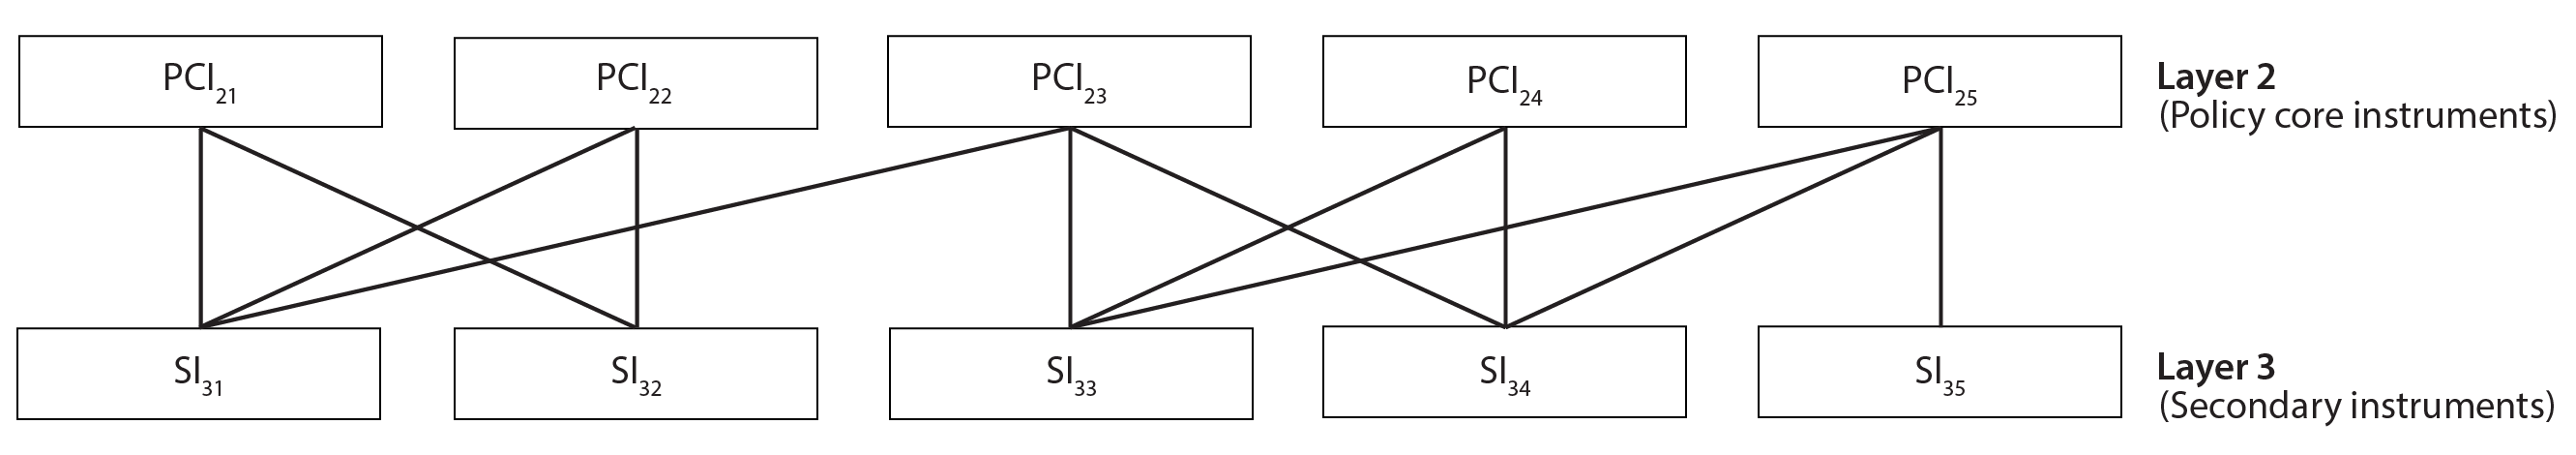
\includegraphics[scale = 0.33, angle = 0]{figures/BeliefTreeConceptualisation-03}
\caption{Conceptual representation of the policy tree hierarchy.}
\label{fig:BeliefTreeConceptualisation-03}
\end{figure} 

The relation between this policy tree for the three streams theory and the policy instruments used for the other theories is as follows. The other theories symply only use the third later of this tree. Furthermore, for them, the impact of each of the secondary instrument is fixed based on modeller inputs.

%
\subsection{The teams - Three streams theory}
\label{ssec:teams3S}

The team concept is another that is incompatible with the different theories. Teams are specifically mentioned in the policy entrepreneurship model which is related to the three streams theory. Teams are therefore considered for the three streams theory part of the model. The teams are built by active actors that feel strongly for an issue they have selected (may it be a problem or a policy). Actors in such a situation will look for other actors in their network for which they think they have similar beliefs. They will then combine their resources to better influence other actors. These teams are short term groups that only last until they have achieved their goal. Actors which do not share the beliefs of a team can leave a team at any time. Actors without a team can also join a team at any time. Actors can only participate in one a team at a time.

The teams have a certain amount of resources. These resources are provided by the actors that are a part of the team. The amount of resources each actor provides the team depends on how close the actor feels belief wise to the team. this is defined as the belonging level. The resources an actor shares with a team is removed from its own resources for other actions. The team leader of the team is always the actor that started the team. Joining a team leads to the exchange of beliefs between the different actors about each other's beliefs on the issue that the team is concerned with. 

%
\subsection{The coalitions - Advocacy coalition framework}
\label{ssec:coalitionACF}

The coalition concept is similar to the team concepts as it is only useful for the ACF. Coalitions are not constructed the same way as teams and no actor can leave a coalition. Coalitions are created based on similar principle beliefs (layer 1) in the agenda setting phase and policy core beliefs (layer 2) in the policy formulation. Initially, the modeller chooses one principle belief for which (s)he judges the coalition should be formed around. Then, the actors with similar beliefs are grouped together in coalitions. The amount of coalitions present in the model is dependent on the threshold that the modeller considers to be similar beliefs. Using a lax definition will lead to only a few coalitions while using a strict definition of similar belief will lead to a fragmented system with numerous coalitions. The belonging level of the actors is calculated after they have been assigned to a coalition. Changes in coalitions are unlikely considering the change in principle beliefs is limited. When joining a coalition, the members of the coalition will all exchange their beliefs so that they understand where everyone stands with respect to the issue advocated by the coalition.

%
\subsection{The Feedback Effects - Feedback theory}
\label{ssec:feedbackEffectsFeedback}

The feedback effects related to the feedback theory can only be considered when the feedback theory is included. This is considered as an extension to the three streams theory and the ACF. Each policy instrument introduced by the modeller can be associated with a specific feedback effect that will have an effect on the structure of the model. These effects are not necessarily known to the actors when they make their choice for a policy instrument. Once a policy instrument has been decided on and is implemented, then the effect is introduced in the technical model at once or over time. Such effect can lead to a change in the provided resources for specific actors or the removal of certain issues from the decision making power of the actors present in the model.
 
Three feedback effects are conceptualised: the meaning of citizenship, the power of groups, and the political agendas and the definition of the policy agenda. According to \cite{mettler2014policy}, the meaning of citizenship feedback effect affects the number of people in some of the sectors of the electorate. The impact of a policy instrument with such a feedback will therefore be a change in the composition of the electorate. The expectation is that will have an impact on the influence that the electorate has on certain policy makers and an impact on the distribution of resources to the actors. The power of groups feedback process is one that affects the policy entrepreneurs. Depending on their affiliation, which is in this case related to the implemented policy, the policy entrepreneurs will have a rise of decrease in the resources their receive throughout the policy emergence process. The exact value and which policy entrepreneurs are impacted the most can be specified by the modeller within the feedback effect of the policy instrument. The political agenda and the definition of the policy agenda feedback mechanism affects what is considered to be within the public realm or the private realm, \cite{mettler2014policy}. Conceptually, if a specific policy instrument has for effect to privatise elements of the system, then some policies and/or problems will have to be removed from the model. The opposite is also true. This feedback effect therefore affects what policies and problems can be considered within the scope of the model.

%
\subsection{The Systems - Diffusion theory}
\label{ssec:SystemsDiffusion}

\textcolor{red}{[WRITE]}

Mention the status of the systems. This is only useful for diffusion and relate to the relative power between the different systems.

%
\subsection{The Super-Policy Network - Diffusion theory}
\label{ssec:superPolicyNetworkDiffusion}

The super-policy network concept is a concept that is compatible with the other theories but that is not useful. This is due to the fact that the diffusion theory can be considered more as an extension to either the three streams theory and the ACF than a model of its own. The diffusion theory requires a set of different systems. These systems can represent different countries or states in which there is a policy emergence process. The diffusion theory helps understand how each of these systems can influence each other.

\begin{figure}
\centering
\includegraphics[scale = 0.33, angle = 0]{figures/Conceptualisation_V3-02}
\caption{Illustration of the policy network and super-policy network for a three systems each using 3-step models.}
\label{fig:Conceptualisation_V3-02}
\end{figure}

This influence is approached through the use of a super-policy network. This is a mirror of the policy network but at the system level. It connects agents present in different systems. This super-policy network is illustrated in \autoref{fig:Conceptualisation_V3-02}. The super-policy networks connects actors in different systems in the same way the policy network connects different actors within one system. Each of these systems has its own policy emergence process which can be influenced by other systems through diffusion mechanisms.

The super-policy network is composed of directed links. They are four types of directed links: friendly, dominant, competitive and coercive. The size of the network is sparser than the policy network with a larger proportion of inactive links. Furthermore, as is shown in \cite{gray1973innovation, walker1969diffusion}, geography is an important factor when considering diffusion mechanisms. The links of the super-policy network therefore have an additional attribute which is the distance between the two actors geographically. This distance will affect the impact of any of their actions. Distant actors being part of two distant systems will have a much lower impact on each other than actors present in close-by systems. This distance attribute can be temporarily changed when external events such as Mayor's conference brings actors to the same geographical location, increasing the potential for impactful actions.
 
%%
\section{The External Events}
\label{sec:externalEvents}
 
The external have an important place within the different theories and the policy emergence process. They can help influence the outcome of the entire process. The external events conceptualised in this thesis have to all be designed by the modeller depending on the intended consequences. Depending on the external events placed, the amount of resources per actor will change or there will be an addition of several policies within the model. The list of class of external events is extensive. The idea behind external events is that if the modeller can think of a specific situation from a case study for example, it should be translated into a model external event. A list of potential external events is presented below. Note that the external events presented below could also be combined or triggered at the same time. This list is not exhaustive:
 
\begin{enumerate}
\item Election: This will have an impact on the representation attributes of the electorate which has a spill-off effect on the resources of the policy maker, policy entrepreneurs and external parties.
\item The introduction of a new issue: This would allow actors to have access to a new issue within their belief tree which they can advocate for.
\item Resource shift: A change in the resource distribution within the model could be designed. This could help represent a power play within the model.
\item Policy network shift: Due to some unknown force, there would be a change in the awareness level of all actors turning some active links inactive and vice-versa.
\item Affiliation network shift: The weights used to describe the relations between the affiliation could be modified.
\item Introduction of a new actor: This would introduce a new actor along with its associated policy network links, beliefs and other attributes.
\item Understanding shift: This would introduce a large change in the causal relations of the different actors present in the model.
\end{enumerate}


